\documentclass{beamer}
\usepackage[utf8]{inputenc}
\usepackage[spanish]{babel}
\usepackage{amsmath}
\usepackage{graphicx}

\usetheme{Madrid}
\usecolortheme{whale}

\title[Modelos Comparativos]{Módulo 4: Aprendizaje Automático}
\subtitle{Clase 5: Taller Comparativo de Algoritmos de Clasificación}
\author{Diplomado en Ciencia de Datos}
\date{\today}

\begin{document}

\begin{frame}
    \titlepage
\end{frame}

% ---------------------------------------------------
\begin{frame}{Objetivos de la Sesión}
    \begin{itemize}
        \item Comprender que no existe un "algoritmo perfecto" (\textit{No Free Lunch Theorem}).
        \item Estudiar \textbf{k-Nearest Neighbors (k-NN)} y el aprendizaje basado en distancia geométrica.
        \item Entender la lógica de los \textbf{Árboles de Decisión} a través de las métricas de partición (Entropía y Gini).
        \item Introducir \textbf{Naive Bayes}, un clasificador puramente probabilístico.
        \item Aprender a implementar cada modelo usando Scikit-Learn y comparar sus resultados.
    \end{itemize}
\end{frame}

% ---------------------------------------------------
\begin{frame}{1. k-Nearest Neighbors (k-NN)}
    \textbf{¿Qué es?} Un algoritmo de aprendizaje "perezoso" (\textit{lazy learning}). No construye una ecuación matemática en el entrenamiento; simplemente memoriza la base de datos.
    \vspace{0.3cm}
    
    \textbf{Mecanismo de Decisión:}
    \begin{itemize}
        \item Cuando llega un nuevo registro, el algoritmo calcula su \textbf{Distancia Euclidiana} hacia todos los puntos existentes.
        \item Selecciona los \textit{k} puntos más cercanos (ej. $k=5$).
        \item La clase mayoritaria entre esos vecinos determina la predicción.
    \end{itemize}
\end{frame}

\begin{frame}{1. k-Nearest Neighbors (Visualización)}
    \begin{center}
        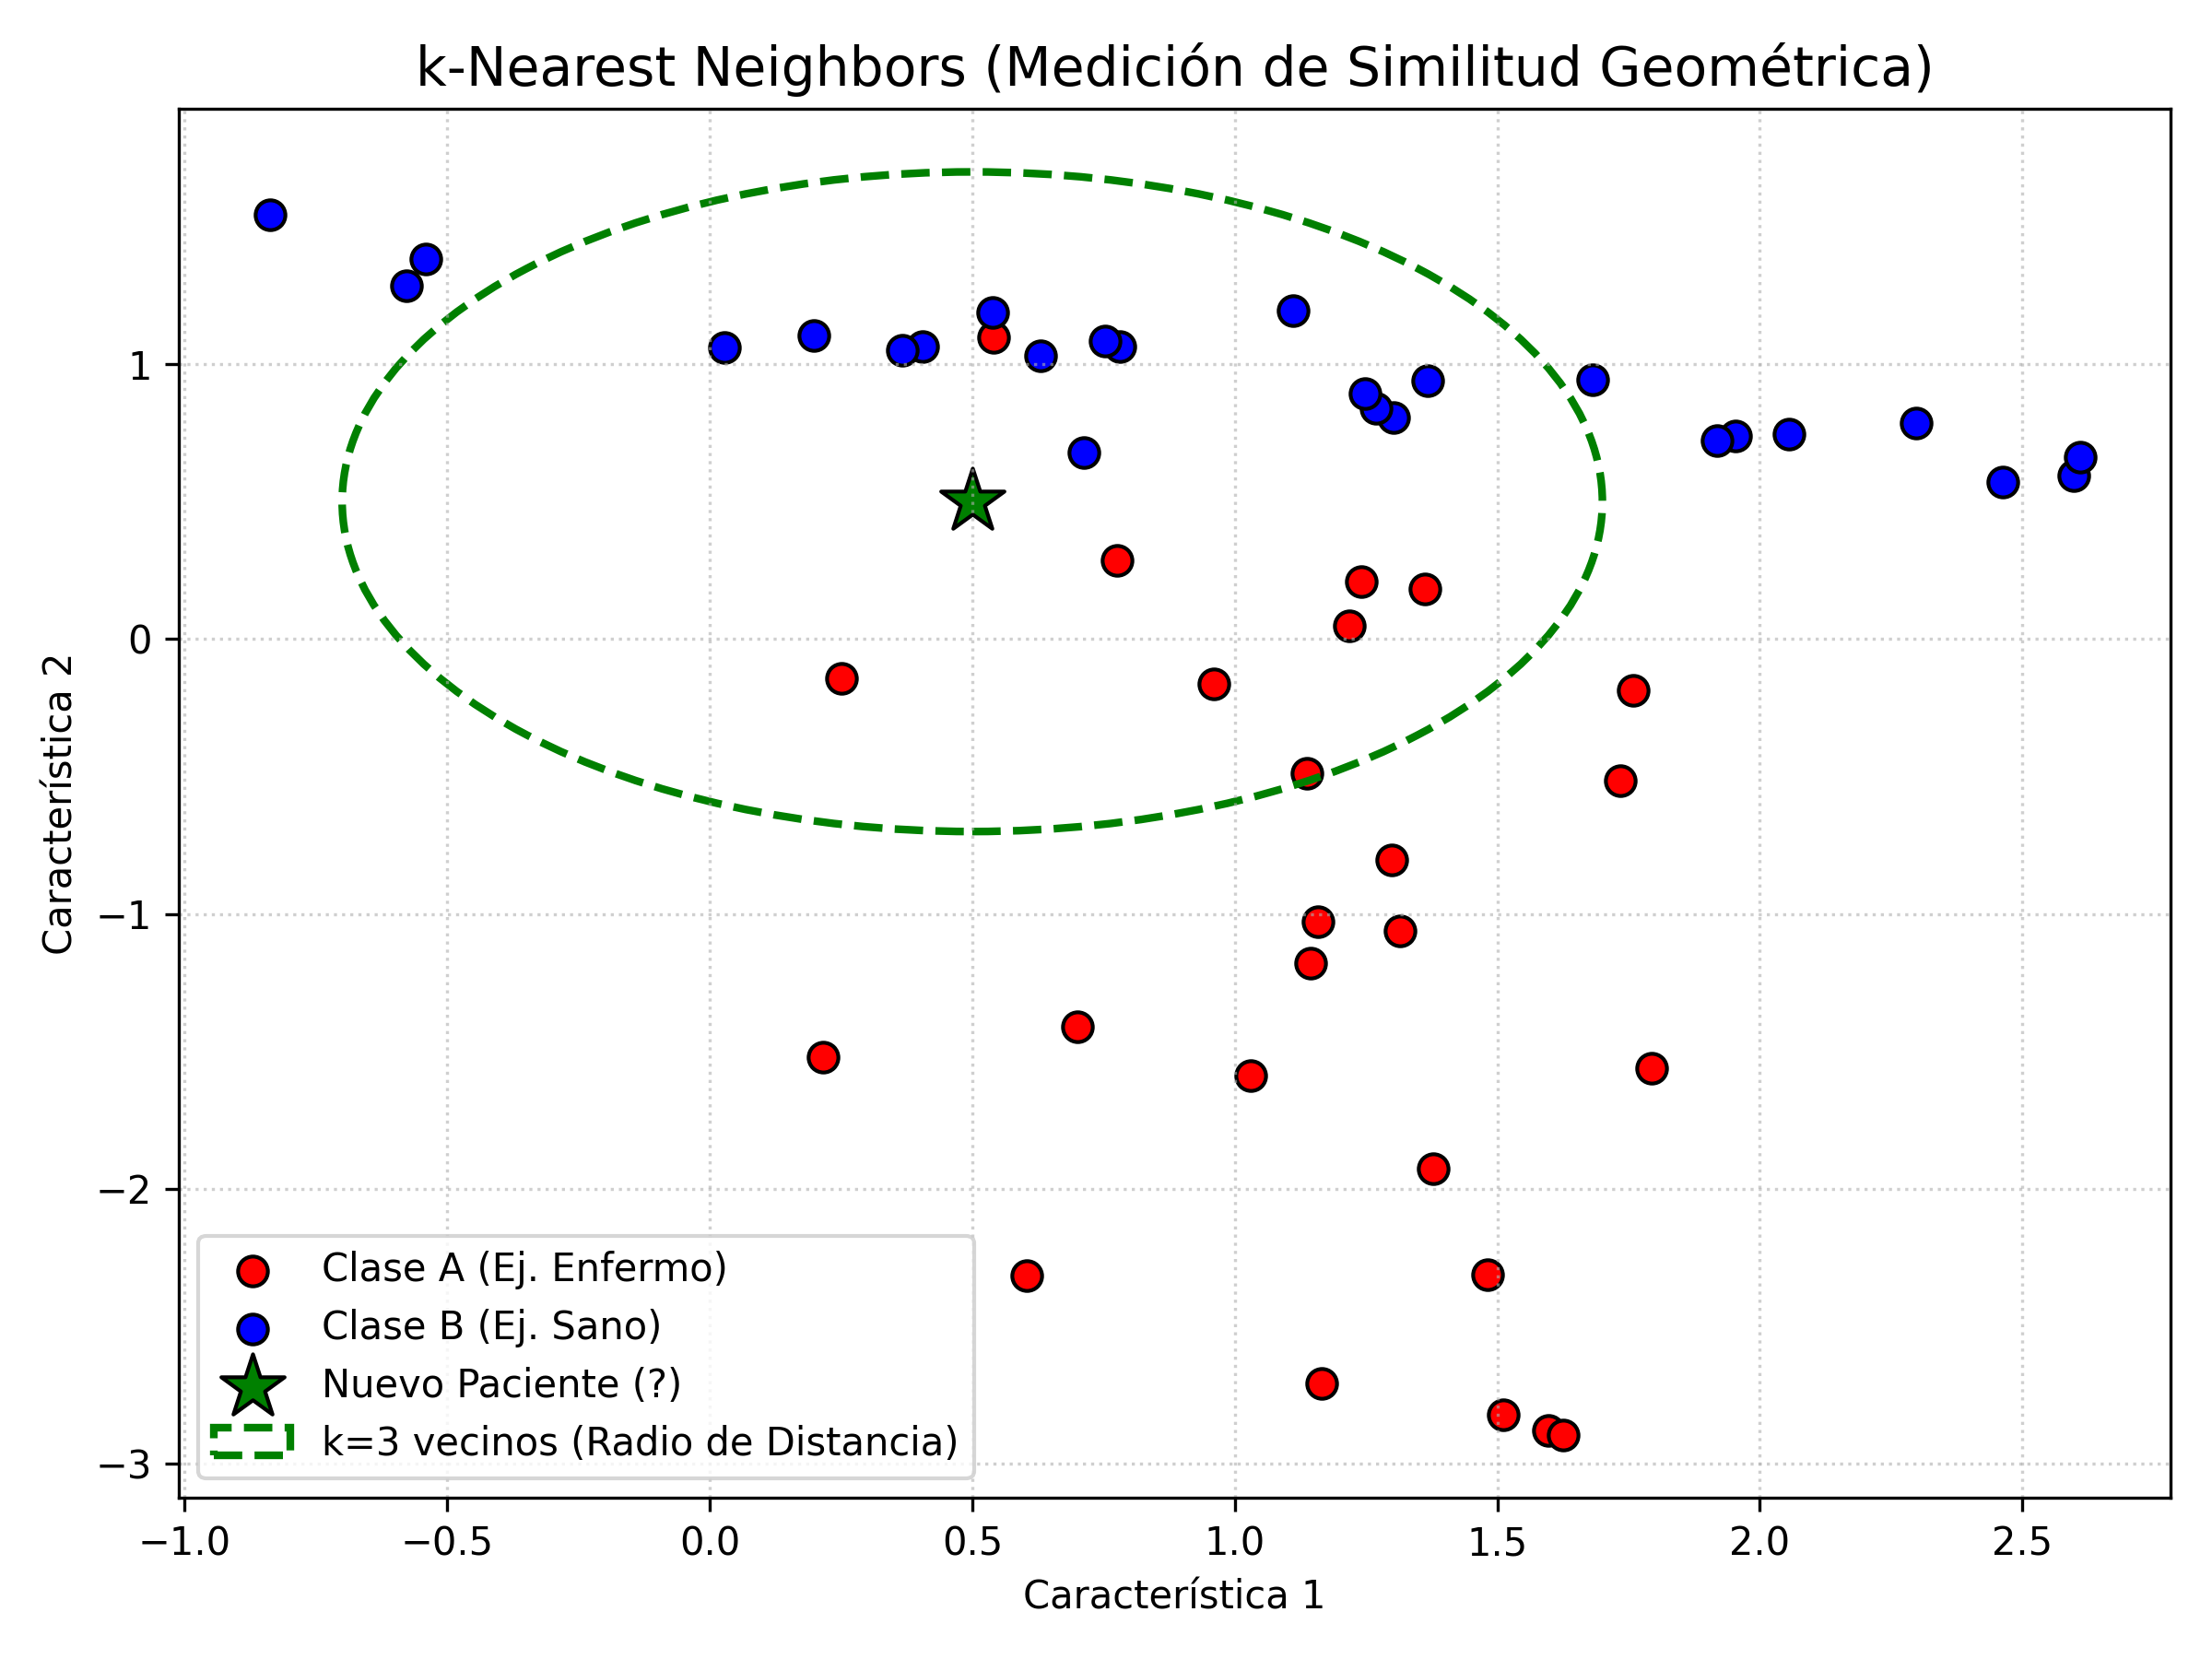
\includegraphics[width=0.85\textwidth,height=0.75\textheight,keepaspectratio]{knn_ejemplo.png}
    \end{center}
\end{frame}

\begin{frame}[fragile]{1. k-NN: Implementación y Precauciones}
    \textbf{Advertencia Crítica:} Debido a que usa distancias geométricas, es obligatorio \textbf{Estandarizar (Escalar)} los datos. Si una columna tiene números muy grandes (ej. Sueldo en miles), dominará el cálculo de distancia.
    
    \vspace{0.3cm}
    \textbf{Comandos Scikit-Learn:}
    \begin{verbatim}
from sklearn.preprocessing import StandardScaler
from sklearn.neighbors import KNeighborsClassifier

# Estandarización obligatoria
scaler = StandardScaler()
X_train_esc = scaler.fit_transform(X_train)

# Instanciación y Entrenamiento
modelo_knn = KNeighborsClassifier(n_neighbors=5)
modelo_knn.fit(X_train_esc, y_train)
    \end{verbatim}
\end{frame}

% ---------------------------------------------------
\begin{frame}{2. Árboles de Decisión}
    \textbf{¿Qué es?} Un modelo basado en reglas lógicas condicionales (\textit{If-Then}). Es altamente intuitivo y fácil de explicar a perfiles de negocio.
    \vspace{0.3cm}
    
    \textbf{Mecanismo de Partición (Splitting):}
    \begin{itemize}
        \item \textbf{Entropía:} Mide el nivel de desorden o impureza en un nodo.
        \item \textbf{Ganancia de Información:} El árbol evaluará todas las variables y cortará los datos usando la pregunta que maximice la ganancia de información (es decir, la pregunta que separe mejor las clases y reduzca la entropía).
        \item También se suele utilizar el Índice \textbf{Gini} como alternativa a la Entropía por ser computacionalmente más rápido.
    \end{itemize}
\end{frame}

\begin{frame}{2. Árboles de Decisión (Visualización)}
    \begin{center}
        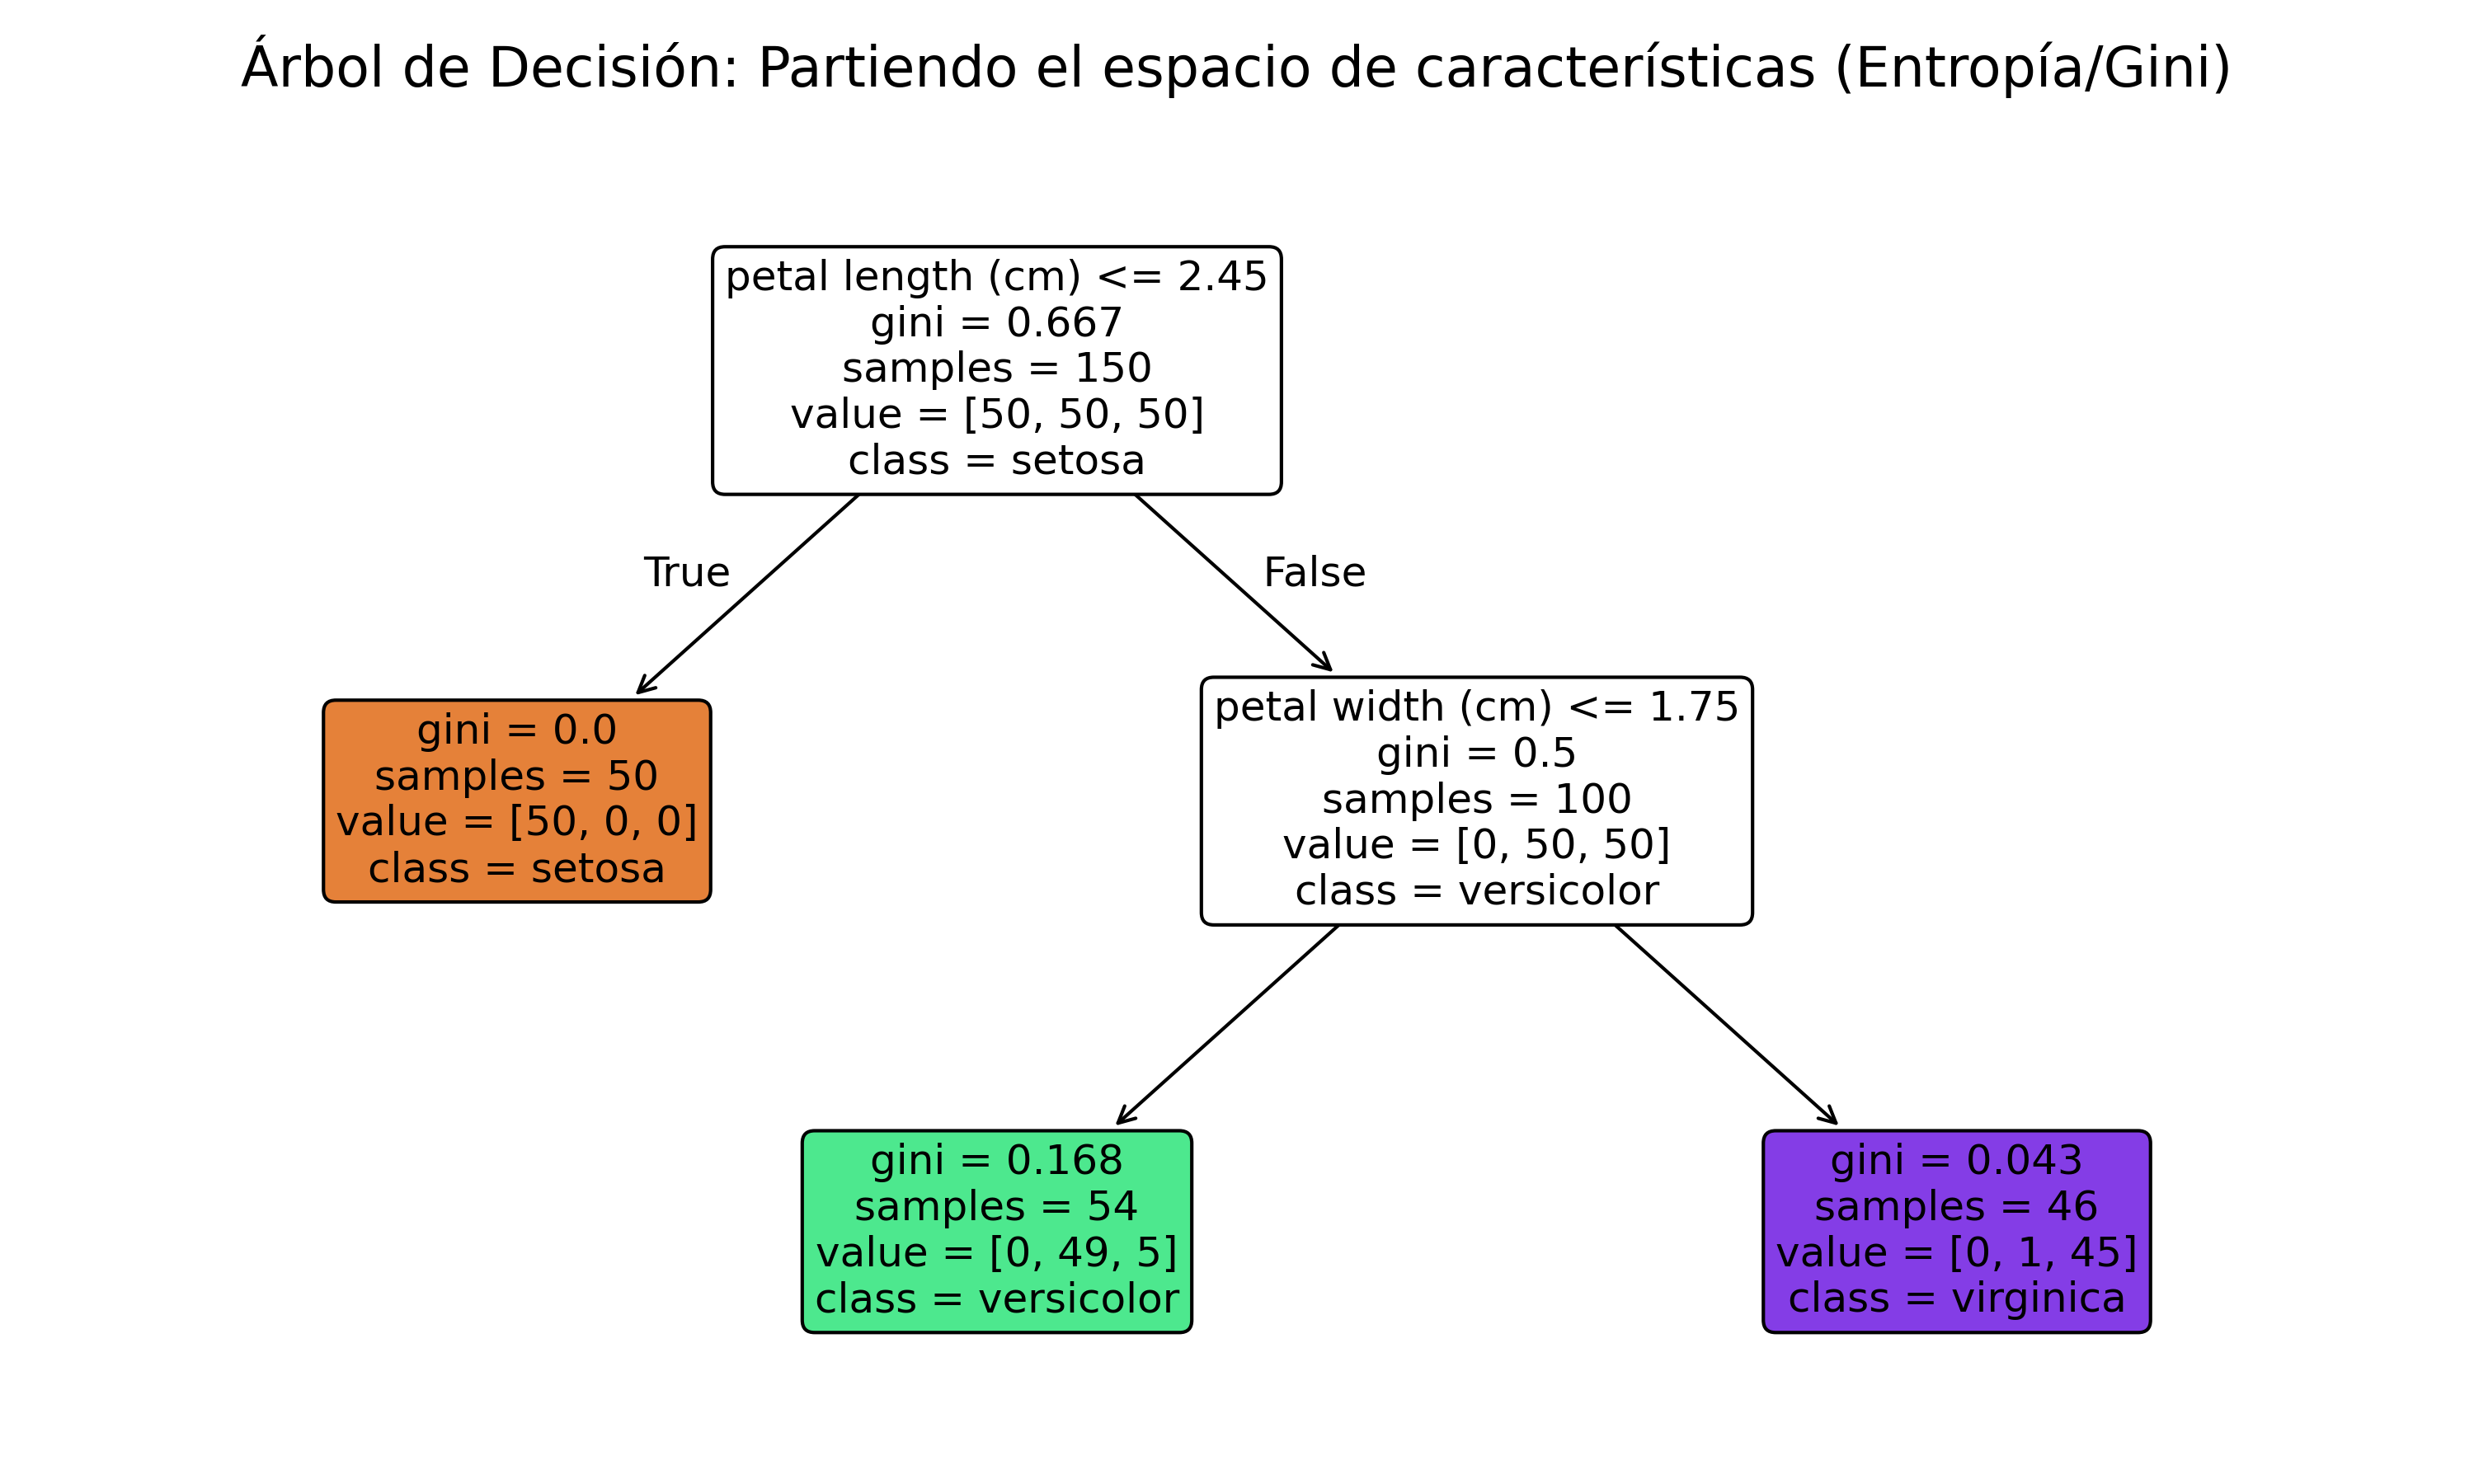
\includegraphics[width=0.9\textwidth,height=0.8\textheight,keepaspectratio]{arbol_ejemplo.png}
    \end{center}
\end{frame}

\begin{frame}[fragile]{2. Árboles: Implementación y Precauciones}
    \textbf{El Peligro del Sobreajuste (Overfitting):} Si no limitamos su crecimiento, el árbol seguirá haciendo preguntas hasta tener una rama para cada registro individual, memorizando los datos pero perdiendo capacidad de generalizar con datos futuros.
    
    \vspace{0.3cm}
    \textbf{Comandos Scikit-Learn:}
    \begin{verbatim}
from sklearn.tree import DecisionTreeClassifier
from sklearn.tree import plot_tree # Para graficar el árbol

# Instanciación (Es vital limitar la profundidad max_depth)
modelo_arbol = DecisionTreeClassifier(max_depth=4, 
                                      criterion='entropy', 
                                      random_state=42)

# Entrenamiento (No requiere escalado previo)
modelo_arbol.fit(X_train, y_train)
    \end{verbatim}
\end{frame}

% ---------------------------------------------------
\begin{frame}{3. Naive Bayes}
    \textbf{¿Qué es?} Un modelo de clasificación basado en el Teorema de Bayes sobre probabilidad condicional.
    \vspace{0.3cm}
    
    \textbf{¿Por qué "Ingenuo" (Naive)?}
    \begin{itemize}
        \item Asume la independencia condicional fuerte. Supone que la presencia de una característica en particular no está relacionada con la presencia de ninguna otra característica.
        \item En la realidad, las variables suelen estar correlacionadas, pero hacer esta asunción "ingenua" simplifica drásticamente el cálculo matemático.
        \item \textbf{Ventajas:} Es extremadamente veloz, ideal para datasets con muchísimas dimensiones (ej. Análisis de texto o detección de Spam).
    \end{itemize}
\end{frame}

\begin{frame}{3. Naive Bayes (Visualización Probabilística)}
    \begin{center}
        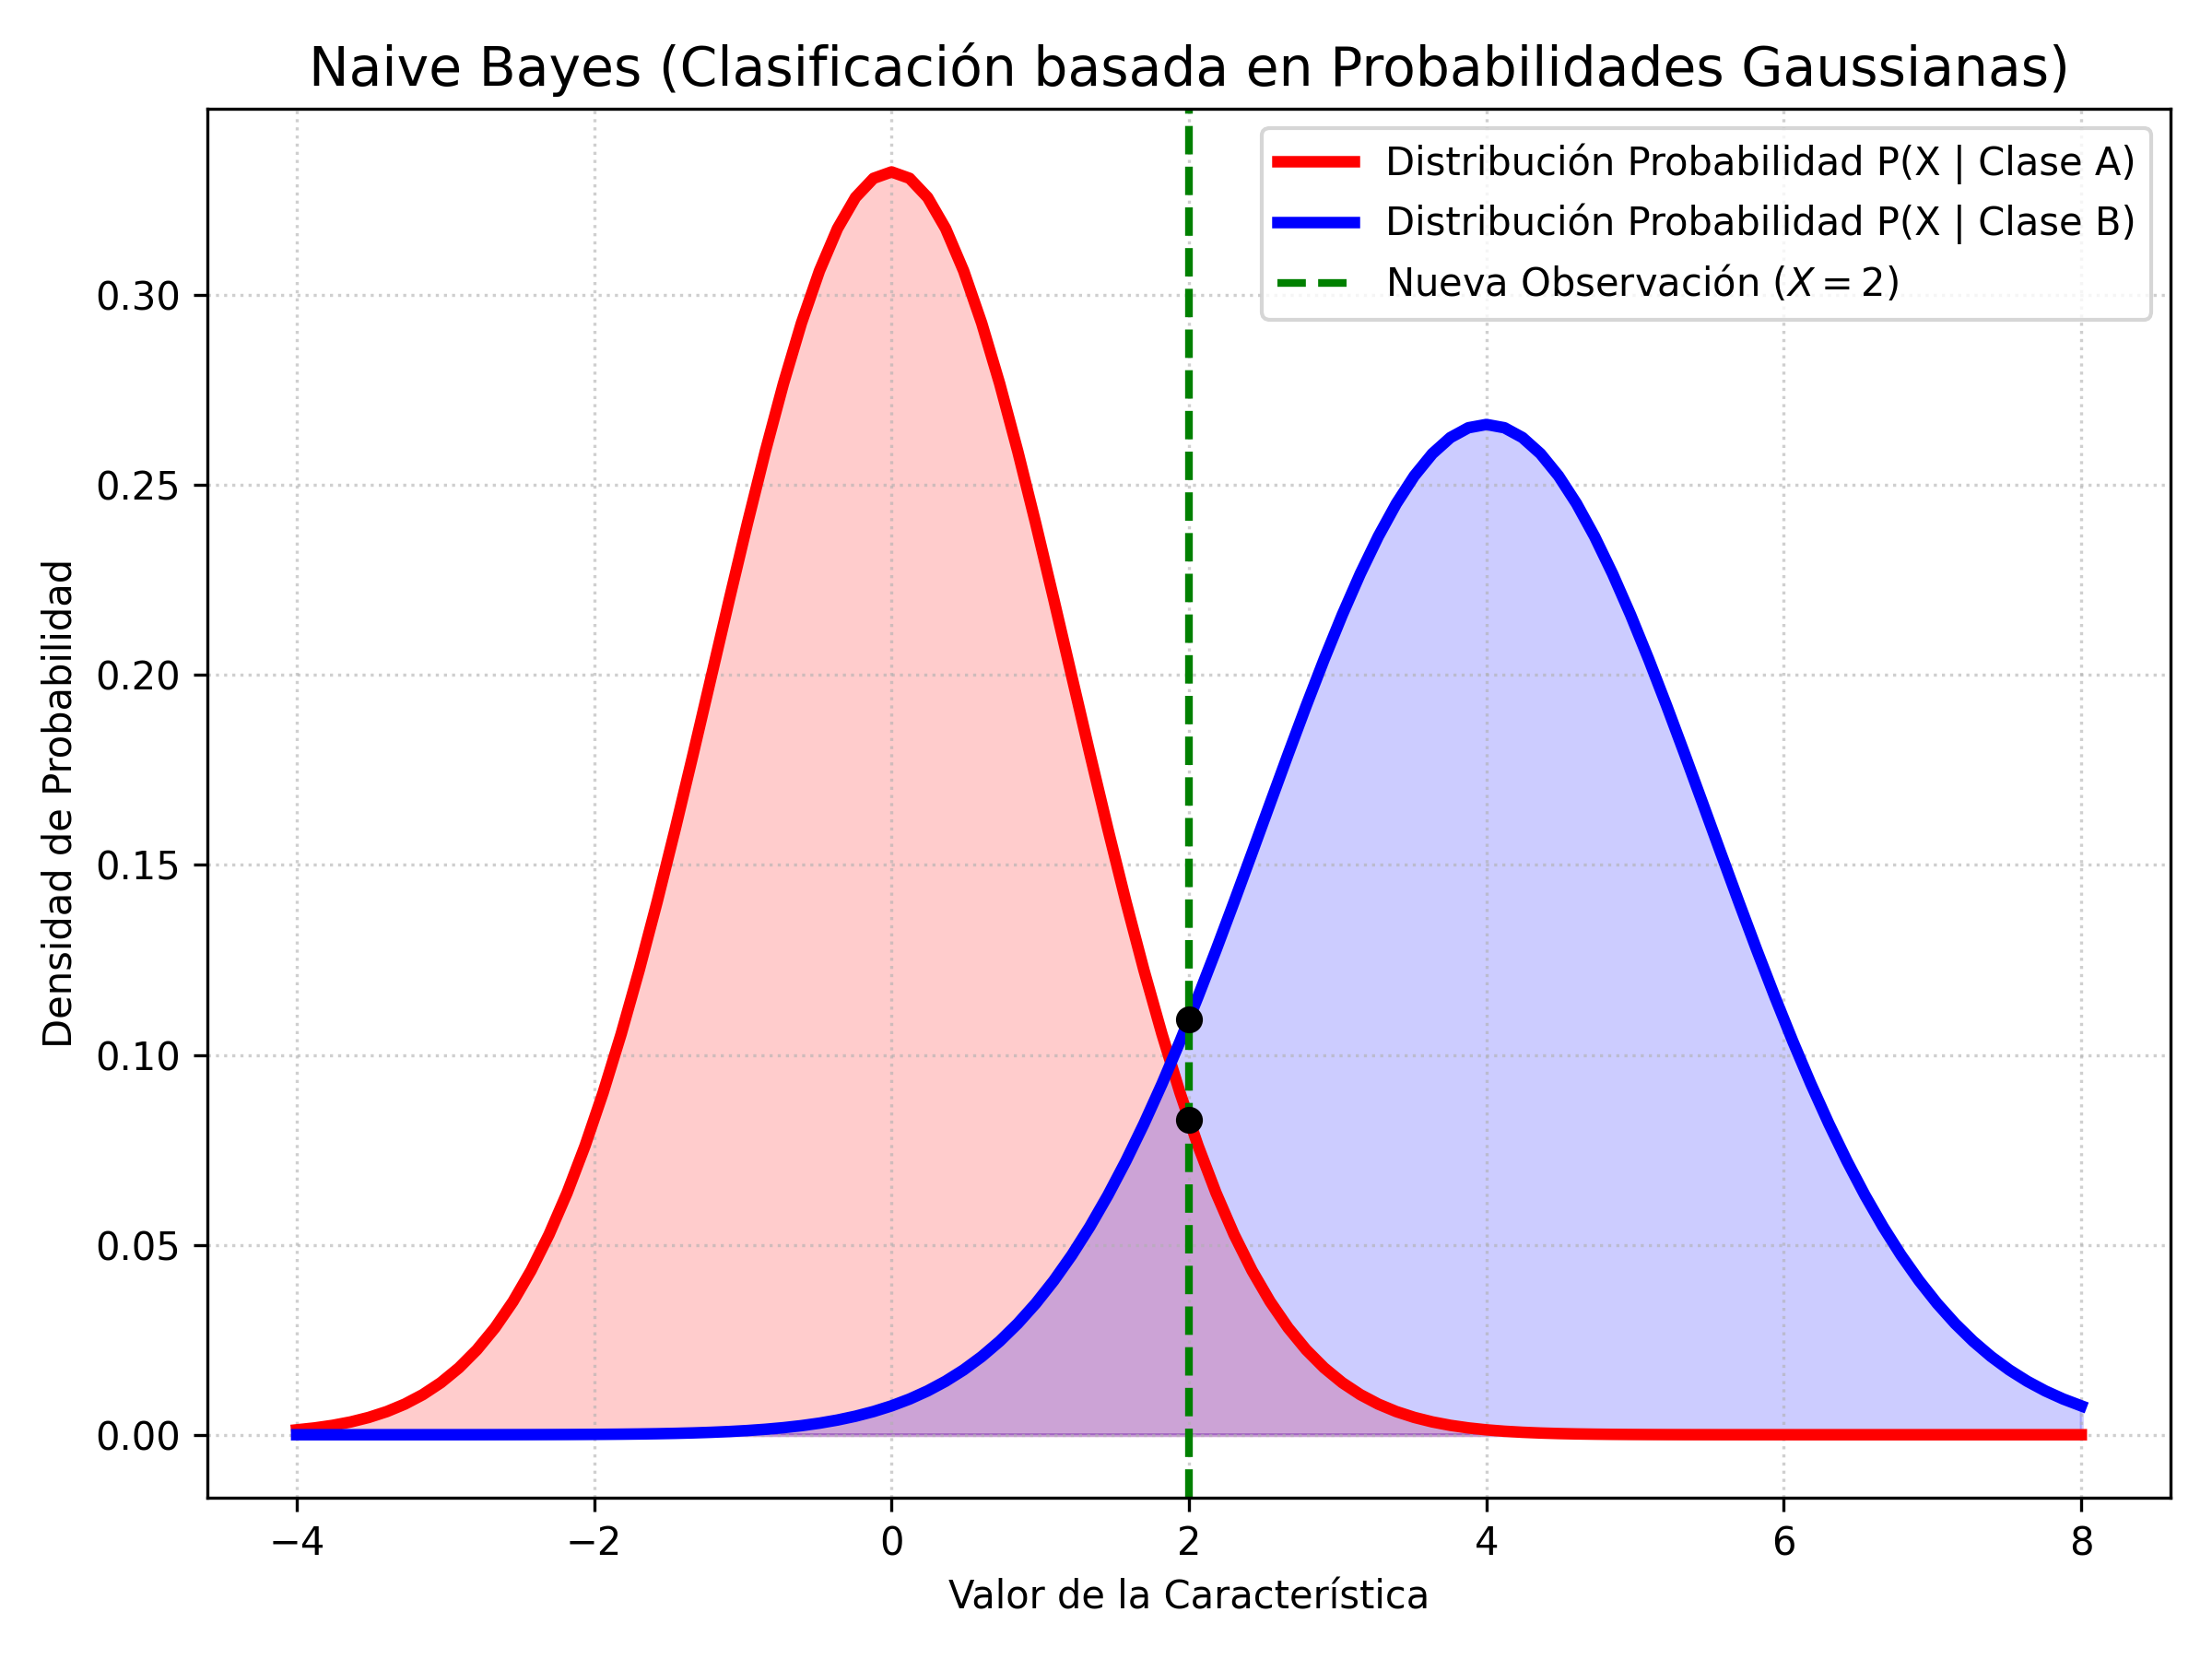
\includegraphics[width=0.85\textwidth,height=0.75\textheight,keepaspectratio]{bayes_ejemplo.png}
    \end{center}
\end{frame}

\begin{frame}[fragile]{3. Naive Bayes: Implementación}
    Existen varias implementaciones (Multinomial para conteo de palabras, Bernoulli para binarios). Para variables continuas del mundo físico usamos \textbf{Gaussian Naive Bayes}.
    
    \vspace{0.3cm}
    \textbf{Comandos Scikit-Learn:}
    \begin{verbatim}
from sklearn.naive_bayes import GaussianNB

# Instanciación
modelo_bayes = GaussianNB()

# Entrenamiento
modelo_bayes.fit(X_train, y_train)

# Predicción
predicciones = modelo_bayes.predict(X_test)
    \end{verbatim}
\end{frame}

% ---------------------------------------------------
\begin{frame}{Torneo de Clasificadores}
    \begin{table}[]
    \centering
    \begin{tabular}{|p{2.5cm}|p{2.5cm}|p{2.5cm}|p{2cm}|}
    \hline
    \textbf{Algoritmo} & \textbf{Ventaja} & \textbf{Desventaja} & \textbf{¿Escalar?} \\ \hline
    \textbf{k-NN} & Excelente con fronteras no lineales & Sufre con muchas variables (Lento) & \textbf{Sí} (Obligatorio) \\ \hline
    \textbf{Decision Tree} & Muy interpretable (Visual) & Alta tendencia al Sobreajuste & No \\ \hline
    \textbf{Naive Bayes} & Ultra veloz, genial para texto & Pierde precisión si hay correlación & No \\ \hline
    \end{tabular}
    \end{table}
\end{frame}

\begin{frame}[fragile]
    \begin{center}
        \Large \textbf{Fin de la Presentación Teórica}\\
        \vspace{0.5cm}
        \normalsize Transición al Laboratorio Práctico Comparativo:\\
        \vspace{0.2cm}
        \verb|05_Comparacion_Clasificadores.ipynb|\\
        \vspace{0.2cm}
        \verb|05_Laboratorio_Evaluacion.ipynb|
    \end{center}
\end{frame}

\end{document}
